\section{استراتژی ایندکس‌گذاری و تحلیل عملکرد}
\label{sec:indexing}

\subsection{اصل طراحی}

هر ایندکس در \Rl{sql/03_indexes.sql} به یک شرط \lr{WHERE}/\lr{ORDER BY}/\lr{JOIN} مشخص در یکی از هشت سناریوی بخش \ref{sec:scenarios} وصل است. هیچ ایندکسی «برای احتیاط» اضافه نشده، چون هر ایندکس هزینه‌ی نوشتاری (رکورد \lr{WAL}، شکافتن صفحه، کار \lr{autovacuum}) به هر \lr{INSERT}/\lr{UPDATE} بعدی آن جدول اضافه می‌کند. همه‌ی شش ایندکس زیر بعد از بارگذاری انبوه (بخش‌های قبلی) ساخته می‌شوند -- همان ترتیب معمول «اول بارگذاری، بعد ایندکس».

\subsection{شش ایندکس هدفمند}

\begin{latin}
\begin{lstlisting}[language=SQL, caption={sql/03\_indexes.sql -- summary}]
-- 1. Composite GIN: title_type (scalar, via btree_gin) + genres (array).
CREATE INDEX idx_title_basics_type_genres_gin
    ON imdb.title_basics USING GIN (title_type, genres);

-- 2. Partial B-tree, scoped to movies -- serves scenario 4.
CREATE INDEX idx_title_basics_movie_year
    ON imdb.title_basics (start_year) WHERE title_type = 'movie';

-- 3. Partial B-tree, scoped to movies with a known runtime -- scenario 8.
CREATE INDEX idx_title_basics_movie_runtime
    ON imdb.title_basics (runtime_minutes)
    WHERE title_type = 'movie' AND runtime_minutes IS NOT NULL;

-- 4. Partial B-tree for Top-N by votes -- scenario 2.
CREATE INDEX idx_title_ratings_votes_desc
    ON imdb.title_ratings (num_votes DESC) WHERE num_votes >= 1000;

-- 5. Partial composite B-tree, scoped to acting credits -- scenario 5.
CREATE INDEX idx_title_principals_cast
    ON imdb.title_principals (nconst, tconst)
    WHERE category IN ('actor', 'actress');

-- 6. Partial composite B-tree, scoped to numbered episodes -- scenario 6.
CREATE INDEX idx_title_episode_parent
    ON imdb.title_episode (parent_tconst, season_number)
    WHERE season_number IS NOT NULL;
\end{lstlisting}
\end{latin}

\paragraph{ایندکس \lr{1} (\lr{GIN} ترکیبی).} سناریوهای \lr{1}، \lr{3}، \lr{5} و \lr{7} همگی روی \lr{title\_type = 'movie'} فیلتر می‌کنند، اما هیچ‌کدام ژانرها را با مقدار خاصی فیلتر نمی‌کنند -- همه‌ی ژانرهای هر سطر را با \lr{unnest()} باز و بعد گروه‌بندی می‌کنند. یک ایندکس \lr{GIN} فقط برای سؤال «آیا این آرایه شامل مقدار \lr{X} است؟» سریع است، نه برای «همه‌ی مقادیر این آرایه را بده» -- پس یک \lr{GIN} تنها روی \lr{genres} هیچ سودی برای این هشت کوئری ندارد. راه‌حلی که انتخاب کردیم از یک ویژگی مستند \lr{GIN} \cite{pggin} استفاده می‌کند: برخلاف \lr{B-Tree} که فقط ستون اول قابل‌استفاده است، یک ایندکس \lr{GIN} چندستونی را می‌شود با فیلتر روی هرکدام از ستون‌هایش هم استفاده کرد. با ترکیب \lr{title\_type} (با کمک \lr{btree\_gin}) و \lr{genres} در یک ایندکس، همین یک ایندکس هم فیلتر \lr{title\_type = 'movie'} را جواب می‌دهد و هم برای سؤال‌های آینده مثل «همه‌ی فیلم‌های کمدی» رایگان کار می‌کند.

\paragraph{ایندکس‌های \lr{2} و \lr{3} (بازه‌ای، جزئی).} \lr{GIN} مفهوم ترتیب ندارد، پس نمی‌تواند شرط بازه‌ای مثل \lr{>= 2000} را جواب دهد -- \lr{B-Tree} ساختار درست برای این حالت است. شرط \lr{WHERE} جزئی هم دقیقاً همان شرط \lr{title\_type = 'movie'} سناریوهای \lr{4} و \lr{8} را تکرار می‌کند تا برنامه‌ریز مجبور نباشد آن را برای هر سطر دوباره چک کند.

\paragraph{ایندکس \lr{4} (\lr{Top-N}).} این یک مثال کلاسیک «ایندکس برای \lr{Top-N}» است: با این ایندکس، پلن به یک اسکن ایندکسی از بالاترین \lr{num\_votes} به پایین تبدیل می‌شود که هر سطر را برای \lr{title\_type = 'movie'} چک می‌کند و به‌محض رسیدن به \lr{LIMIT 10} متوقف می‌شود -- به‌جای این‌که همه‌ی عنوان‌های امتیازدهی‌شده را مرتب کند.

\paragraph{ایندکس \lr{5} (سنگین‌ترین سناریو).} \lr{category} حدود ده مقدار متفاوت دارد (\lr{actor}، \lr{actress}، \lr{director}، ...)؛ محدودکردن ایندکس به \lr{actor}/\lr{actress} آن را نسبت به کل جدول \lr{~90} میلیون سطری کوچک‌تر می‌کند. ستون اول \lr{nconst} است (همان کلید \lr{GROUP BY} سناریو)، پس اعتبارهای بازیگری یک نفر کنار هم در ایندکس قرار می‌گیرند. کلید اصلی خود \lr{title\_principals}، یعنی \lr{PK(tconst, ordering)}، از قبل یک مسیر بر اساس \lr{tconst} در اختیار برنامه‌ریز می‌گذارد؛ این ایندکس مسیر مکمل بر اساس \lr{nconst} را اضافه می‌کند که سمت \lr{GROUP BY} به آن نیاز دارد.

\paragraph{ایندکس \lr{6}.} \lr{parent\_tconst} هیچ ایندکسی نداشت (فقط \lr{tconst}، کلید اصلی)، پس پیوند به \lr{title\_basics} باعث اسکن کامل \lr{title\_episode} می‌شد.

\paragraph{عمداً بدون ایندکس:} ستون \lr{directors} در جدول \lr{title\_crew}، و یک \lr{GIN} تنها روی \lr{genres}. چون هیچ‌کدام از سناریوها فیلتر \lr{containment} روی این آرایه‌ها ندارند. هر ستون \lr{metadata JSONB} هم همین‌طور: هیچ‌کدام از هشت سناریو آن را نمی‌خواند، و یک ایندکس بدون کوئری فقط هزینه‌ی نوشتاری است.

\subsection{مقیاس داده‌ی اجرای واقعی}
\label{sec:real-data-scale}

این بخش دیگر پیش‌بینی نیست: همه‌چیز را واقعاً روی یک \lr{PostgreSQL 16} داخل \lr{Docker} اجرا و اندازه‌گیری کردیم. یک محدودیت واقعی هم داشتیم که باید صادقانه گفت: لپ‌تاپی که این اجرا رویش انجام شد فقط حدود \lr{30} گیگابایت فضای خالی روی دیسک داشت، و بیشتر از این هم نمی‌شد فضا آزاد کرد. دیتاست کامل \lr{IMDb} -- مخصوصاً جدول \lr{title\_principals} با نزدیک \lr{90} میلیون سطر -- توی این فضا جا نمی‌شد؛ هم خود جدول بزرگ است، هم \lr{WAL} و ایندکس‌هایی که رویش می‌سازیم فضا لازم دارند.

راه‌حلی که استفاده شد: پنج جدول موردنیاز دیگر (\lr{title\_ratings}، \lr{title\_episode}، \lr{title\_crew}، \lr{title\_basics}، \lr{name\_basics}) کامل و بدون هیچ کم‌وکاستی بارگذاری شدند. فقط \lr{title\_principals} -- بزرگ‌ترین جدول -- با فلگ \lr{--limit-rows} همان اسکریپت \Rl{scripts/producer.py} به \lr{8{,}000{,}000} سطر اول محدود شد (حدود \lr{9\%} از حجم واقعی آن). جدول زیر عددهای واقعی هرکدام را نشان می‌دهد:

\begin{table}[h]
\centering
\caption{تعداد سطرهای واقعی بارگذاری‌شده}
\begin{tabular}{@{}lrl@{}}
\toprule
\textbf{جدول} & \textbf{سطر بارگذاری‌شده} & \textbf{وضعیت} \\
\midrule
\lr{title\_ratings}    & \lr{1{,}702{,}067}  & کامل \\
\lr{title\_episode}    & \lr{9{,}808{,}098}  & کامل \\
\lr{title\_crew}       & \lr{12{,}689{,}431} & کامل \\
\lr{title\_basics}     & \lr{12{,}689{,}431} & کامل \\
\lr{name\_basics}      & \lr{15{,}542{,}711} & کامل \\
\lr{title\_principals} & \lr{8{,}000{,}000}  & محدودشده (حدود \lr{9\%} از \lr{~90M} واقعی) \\
\bottomrule
\end{tabular}
\end{table}

یعنی سناریوی \lr{5} -- تنها سناریویی که از \lr{title\_principals} می‌خواند -- روی حجمی کوچک‌تر از واقعیت اجرا شده. بهبود واقعی آن روی دیتاست کامل احتمالاً بیشتر از عددی است که در ادامه می‌بینید. عددهای شش سناریوی دیگر همه روی جدول‌های کامل به‌دست آمده‌اند.

\subsection{روش‌شناسی مقایسه‌ی قبل/بعد}

با این دستورها (دقیقاً همان‌هایی که اجرا شدند):

\begin{latin}
\begin{lstlisting}[language=bash]
python scripts/run_scenarios.py --phase before --repeat 2
docker exec -i imdb_postgres psql -U imdb -d imdb -f - < sql/03_indexes.sql
python scripts/run_scenarios.py --phase after --repeat 2
python scripts/compare_timings.py
\end{lstlisting}
\end{latin}

اسکریپت \Rl{scripts/compare_timings.py} این جدول را می‌سازد. ورودی آن دو دسته فایل واقعی نتیجه است: \Rl{results/timings/scenario_timings.csv} و \Rl{results/explain/*.txt}. خروجی نهایی هم در \Rl{results/comparison.md} نوشته شده است.

\begin{table}[h]
\centering
\caption{نتیجه‌ی واقعی: قبل در برابر بعد از ایندکس‌گذاری}
\scriptsize
\begin{tabular}{@{}rrrrrrp{2.9cm}@{}}
\toprule
\textbf{\#} & \textbf{قبل (ms)} & \textbf{بعد (ms)} & \textbf{تغییر} & \textbf{خواندن (قبل)} & \textbf{خواندن (بعد)} & \textbf{تغییر پلن} \\
\midrule
\lr{1} & \lr{4381.2}   & \lr{8953.3}  & \lr{-104\%} & \lr{249{,}303} & \lr{136{,}532} & \lr{Seq} $\to$ \lr{Bitmap} (کندتر) \\
\lr{2} & \lr{93.0}     & \lr{12.7}    & \lr{+86\%}  & \lr{32}        & \lr{31}        & \lr{Seq+Sort} $\to$ \lr{Index} \\
\lr{3} & \lr{147701.3} & \lr{101420.8}& \lr{+31\%}  & \lr{645{,}775} & \lr{576{,}826} & تغییر نکرد \\
\lr{4} & \lr{10381.5}  & \lr{5224.3}  & \lr{+50\%}  & \lr{261{,}320} & \lr{180{,}000} & \lr{Seq} $\to$ \lr{Bitmap} \\
\lr{5} & \lr{22671.7}  & \lr{15555.8} & \lr{+31\%}  & \lr{223{,}012} & \lr{256{,}022} & \lr{Seq} $\to$ \lr{Index Only} \\
\lr{6} & \lr{34691.0}  & \lr{22079.1} & \lr{+36\%}  & \lr{248{,}270} & \lr{179{,}676} & \lr{Seq} $\to$ \lr{Index Only} \\
\lr{7} & \lr{3852.0}   & \lr{1143.7}  & \lr{+70\%}  & \lr{115{,}524} & \lr{106{,}690} & \lr{Seq} $\to$ \lr{Bitmap} \\
\lr{8} & \lr{2803.6}   & \lr{1930.8}  & \lr{+31\%}  & \lr{115{,}045} & \lr{410}       & \lr{Seq} $\to$ \lr{Bitmap} \\
\bottomrule
\end{tabular}
\end{table}

\begin{figure}[h]
\centering
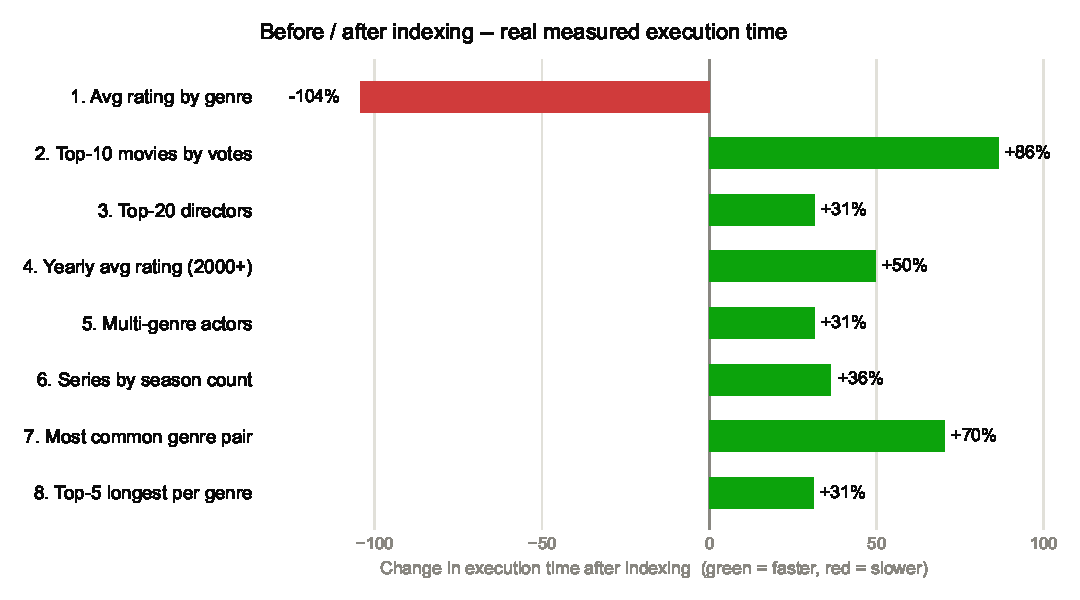
\includegraphics[width=0.85\linewidth]{figures/performance_comparison.pdf}
\caption{همان جدول، به‌صورت نموداری -- درصد تغییر زمان اجرای هر سناریو}
\end{figure}

\paragraph{شش سناریو دقیقاً طبق پیش‌بینی بهتر شدند.} سناریوهای \lr{2}، \lr{4}، \lr{5}، \lr{6}، \lr{7} و \lr{8} همه سریع‌تر شدند. در همه‌ی آن‌ها \lr{Seq Scan} با یک روش ایندکسی (\lr{Index Scan}، \lr{Index Only Scan} یا \lr{Bitmap Heap/Index Scan}) جایگزین شد. بیشترین بهبود مال سناریوی \lr{2} است: از \lr{93} به \lr{12.7} میلی‌ثانیه. ایندکس جزئی \lr{idx\_title\_ratings\_votes\_desc} دقیقاً همان چیزی را می‌دهد که \lr{Top-N} لازم دارد، یعنی مرتب‌سازی کامل حذف می‌شود. نمونه‌ی چشمگیر دیگر سناریوی \lr{8} است: تعداد بلوک خوانده‌شده از دیسک از \lr{115{,}045} به فقط \lr{410} رسید.

\paragraph{سناریوی \lr{3} هنوز کندترین کوئری است -- طبق طراحی.} همان‌طور که در بخش «عمداً بدون ایندکس» گفتیم، هیچ ایندکسی برای ستون \lr{directors} در جدول \lr{title\_crew} نساختیم. این سناریو هم \lr{31\%} سریع‌تر شد، اما این بهبود از خود این تصمیم نیست؛ از تغییری می‌آید که ایندکس‌های \lr{title\_basics} غیرمستقیم روی پیوندهای این کوئری گذاشته‌اند. نکته‌ی جالب این است که این سناریو -- نه سناریوی \lr{5} -- در این اجرا سنگین‌ترین کوئری از آب درآمد. دلیلش همان محدودیت بخش \ref{sec:real-data-scale} است: \lr{title\_crew} و \lr{name\_basics} کامل بارگذاری شدند (\lr{~12.7M} و \lr{~15.5M} سطر)، ولی \lr{title\_principals} فقط \lr{8M} سطر داشت. روی دیتاست کامل \lr{IMDb}، سناریوی \lr{5} احتمالاً دوباره سنگین‌ترین می‌شد، چون از \lr{~90} میلیون سطر \lr{title\_principals} شروع می‌شود.

\paragraph{سناریوی \lr{1} کندتر شد -- و این هم یک نتیجه‌ی واقعی و آموزنده است.} این عدد را مخفی نمی‌کنیم: پلن بعد از ایندکس واقعاً کندتر بود، از \lr{4381} به \lr{8953} میلی‌ثانیه. خود \lr{EXPLAIN} دلیلش را نشان می‌دهد. تعداد بلوک خوانده‌شده از دیسک واقعاً کم شده (از \lr{249{,}303} به \lr{136{,}532})، اما زمان \lr{I/O} واقعی تقریباً دو برابر شده (از حدود \lr{14.9} به \lr{24.9} ثانیه). دلیلش این است که دسترسی از حالت پی‌درپی (در \lr{Parallel Seq Scan}) به دسترسی پراکنده (در \lr{Bitmap Heap Scan}) تغییر کرده.

مشکل اصلی این است که شرط \lr{title\_type = 'movie'} گزینش‌پذیر (\lr{selective}) کافی نیست: نزدیک \lr{30\%} سطرهای \lr{title\_basics} از نوع \lr{movie} هستند. پس \lr{Bitmap Heap Scan} تقریباً به همان تعداد صفحه‌ی دیسک سر می‌زند که یک اسکن کامل می‌زد، ولی با دسترسی پراکنده‌تر و هزینه‌ی اضافه‌ی ساخت بیت‌مپ. درسش ساده است: ایندکس فقط وقتی برنده است که شرط واقعاً گزینشی باشد. روی یک ستون کم‌گزینش مثل \lr{title\_type}، برنامه‌ریز گاهی اشتباه می‌کند؛ برای همین باید همیشه با \lr{EXPLAIN (ANALYZE, BUFFERS)} واقعی تصمیم گرفت، نه فقط با نگاه‌کردن به لیست ایندکس‌ها. (سناریوهای \lr{3}، \lr{5} و \lr{7} هم همین ایندکس \lr{GIN} را برای همین شرط دارند، اما چون شرط دیگری در کوئری‌شان گزینش‌پذیری بیشتری اضافه می‌کند، این اثر منفی آن‌جا دیده نشد.)

\subsection{نمونه‌ی واقعی خروجی \lr{EXPLAIN ANALYZE}}
\label{sec:explain-samples}

خروجی کامل \lr{EXPLAIN (ANALYZE, BUFFERS, SETTINGS)} هر \lr{8} سناریو -- هم قبل و هم بعد از ایندکس‌گذاری، یعنی \lr{16} فایل -- در \Rl{results/explain/} ذخیره شده است. سه نمونه‌ی زیر مستقیماً از همان فایل‌هاست، فقط برای جاشدن در صفحه خلاصه شده‌اند: گره‌های سطح-کارگر و برآورد هزینه‌ی برنامه‌ریز حذف شده‌اند، ولی زمان‌های واقعی و بافرها دست‌نخورده‌اند.

\textbf{سناریوی \lr{1}، قبل و بعد -- همان رگرسیونی که در بالا توضیح داده شد:}

\begin{latin}
\begin{lstlisting}[caption={results/explain/scenario\_01.txt -- BEFORE (excerpt)}]
Sort  (actual time=4347.848..4379.101 rows=27 loops=1)
  Buffers: shared hit=12087 read=249303
  ->  Finalize GroupAggregate  (actual time=4347.418..4378.968 rows=27 loops=1)
        ->  Gather Merge  (Workers Launched: 4)
              ->  Parallel Hash Join  (actual time=2356.150..4191.300 rows=69766 loops=5)
                    ->  Parallel Seq Scan on title_ratings tr
                          (actual time=0.611..1577.639 rows=340413 loops=5)
                    ->  Parallel Seq Scan on title_basics tb
                          Filter: (title_type = 'movie'::text)
                          Rows Removed by Filter: 2387111
                          (actual time=0.596..2089.660 rows=150775 loops=5)
Planning Time: 8.385 ms
Execution Time: 4381.153 ms
\end{lstlisting}
\begin{lstlisting}[caption={results/explain/scenario\_01.after.txt -- AFTER (excerpt)}]
Sort  (actual time=8907.907..8948.027 rows=27 loops=1)
  Buffers: shared hit=69029 read=136532 written=3892
  I/O Timings: shared read=24943.451 write=416.247
  ->  Finalize GroupAggregate  (actual time=8907.699..8947.988 rows=27 loops=1)
        ->  Gather Merge  (Workers Launched: 4)
              ->  Parallel Hash Join  (actual time=6890.573..8659.886 rows=69766 loops=5)
                    ->  Parallel Seq Scan on title_ratings tr
                          (actual time=0.224..1494.175 rows=340413 loops=5)
                    ->  Parallel Bitmap Heap Scan on title_basics tb
                          Recheck Cond: (title_type = 'movie'::text)
                          Heap Blocks: exact=34108
                          (actual time=659.714..6046.800 rows=150775 loops=5)
                          ->  Bitmap Index Scan on idx_title_basics_type_genres_gin
                                (actual time=588.927..588.927 rows=753874 loops=1)
Planning Time: 23.851 ms
Execution Time: 8953.258 ms
\end{lstlisting}
\end{latin}

\textbf{سناریوی \lr{2}، بعد از ایندکس -- بزرگ‌ترین بهبود (از \lr{93} به \lr{12.7} میلی‌ثانیه):}

\begin{latin}
\begin{lstlisting}[caption={results/explain/scenario\_02.after.txt (excerpt)}]
Limit  (actual time=2.379..12.610 rows=10 loops=1)
  Buffers: shared hit=43 read=31
  ->  Nested Loop  (actual time=2.377..12.596 rows=10 loops=1)
        ->  Index Scan using idx_title_ratings_votes_desc on title_ratings tr
              (actual time=1.171..1.235 rows=12 loops=1)
        ->  Index Scan using title_basics_pkey on title_basics tb
              Filter: (title_type = 'movie'::text)
              (actual time=0.939..0.939 rows=1 loops=12)
Planning Time: 7.632 ms
Execution Time: 12.683 ms
\end{lstlisting}
\end{latin}

\textbf{سناریوی \lr{8}، قبل و بعد -- افت بافر خوانده‌شده از \lr{115{,}045} به \lr{410}:}

\begin{latin}
\begin{lstlisting}[caption={results/explain/scenario\_08.txt -- BEFORE, main node only (excerpt)}]
Parallel Seq Scan on title_basics tb  (actual time=2.135..687.571 rows=95056 loops=5)
  Filter: ((runtime_minutes IS NOT NULL) AND (title_type = 'movie'::text))
  Rows Removed by Filter: 2442830
  Buffers: shared hit=115350 read=115044
-- (full plan: Nested Loop -> Sort -> Gather Merge -> WindowAgg above this node)
Execution Time: 2803.599 ms
\end{lstlisting}
\begin{lstlisting}[caption={results/explain/scenario\_08.after.txt (excerpt)}]
Subquery Scan on ranked  (actual time=1079.154..1927.038 rows=135 loops=1)
  Buffers: shared hit=142987 read=410
  ->  WindowAgg  (Run Condition: (row_number() OVER (?) <= 5))
        ->  Nested Loop  (actual time=146.206..477.905 rows=148312 loops=5)
              ->  Parallel Bitmap Heap Scan on title_basics tb
                    Recheck Cond: ((title_type = 'movie'::text) AND
                                    (runtime_minutes IS NOT NULL))
                    (actual time=146.106..382.596 rows=95056 loops=5)
                    ->  Bitmap Index Scan on idx_title_basics_movie_runtime
                          (actual time=91.626..91.626 rows=475280 loops=1)
Planning Time: 5.891 ms
Execution Time: 1930.801 ms
\end{lstlisting}
\end{latin}
